\documentclass{standalone}
\usepackage{tikz}
\usetikzlibrary{patterns, positioning}
\usepackage[sfdefault]{ClearSans} %% option 'sfdefault' activates Clear Sans as the default text font
\usepackage[T1]{fontenc}

\begin{document}
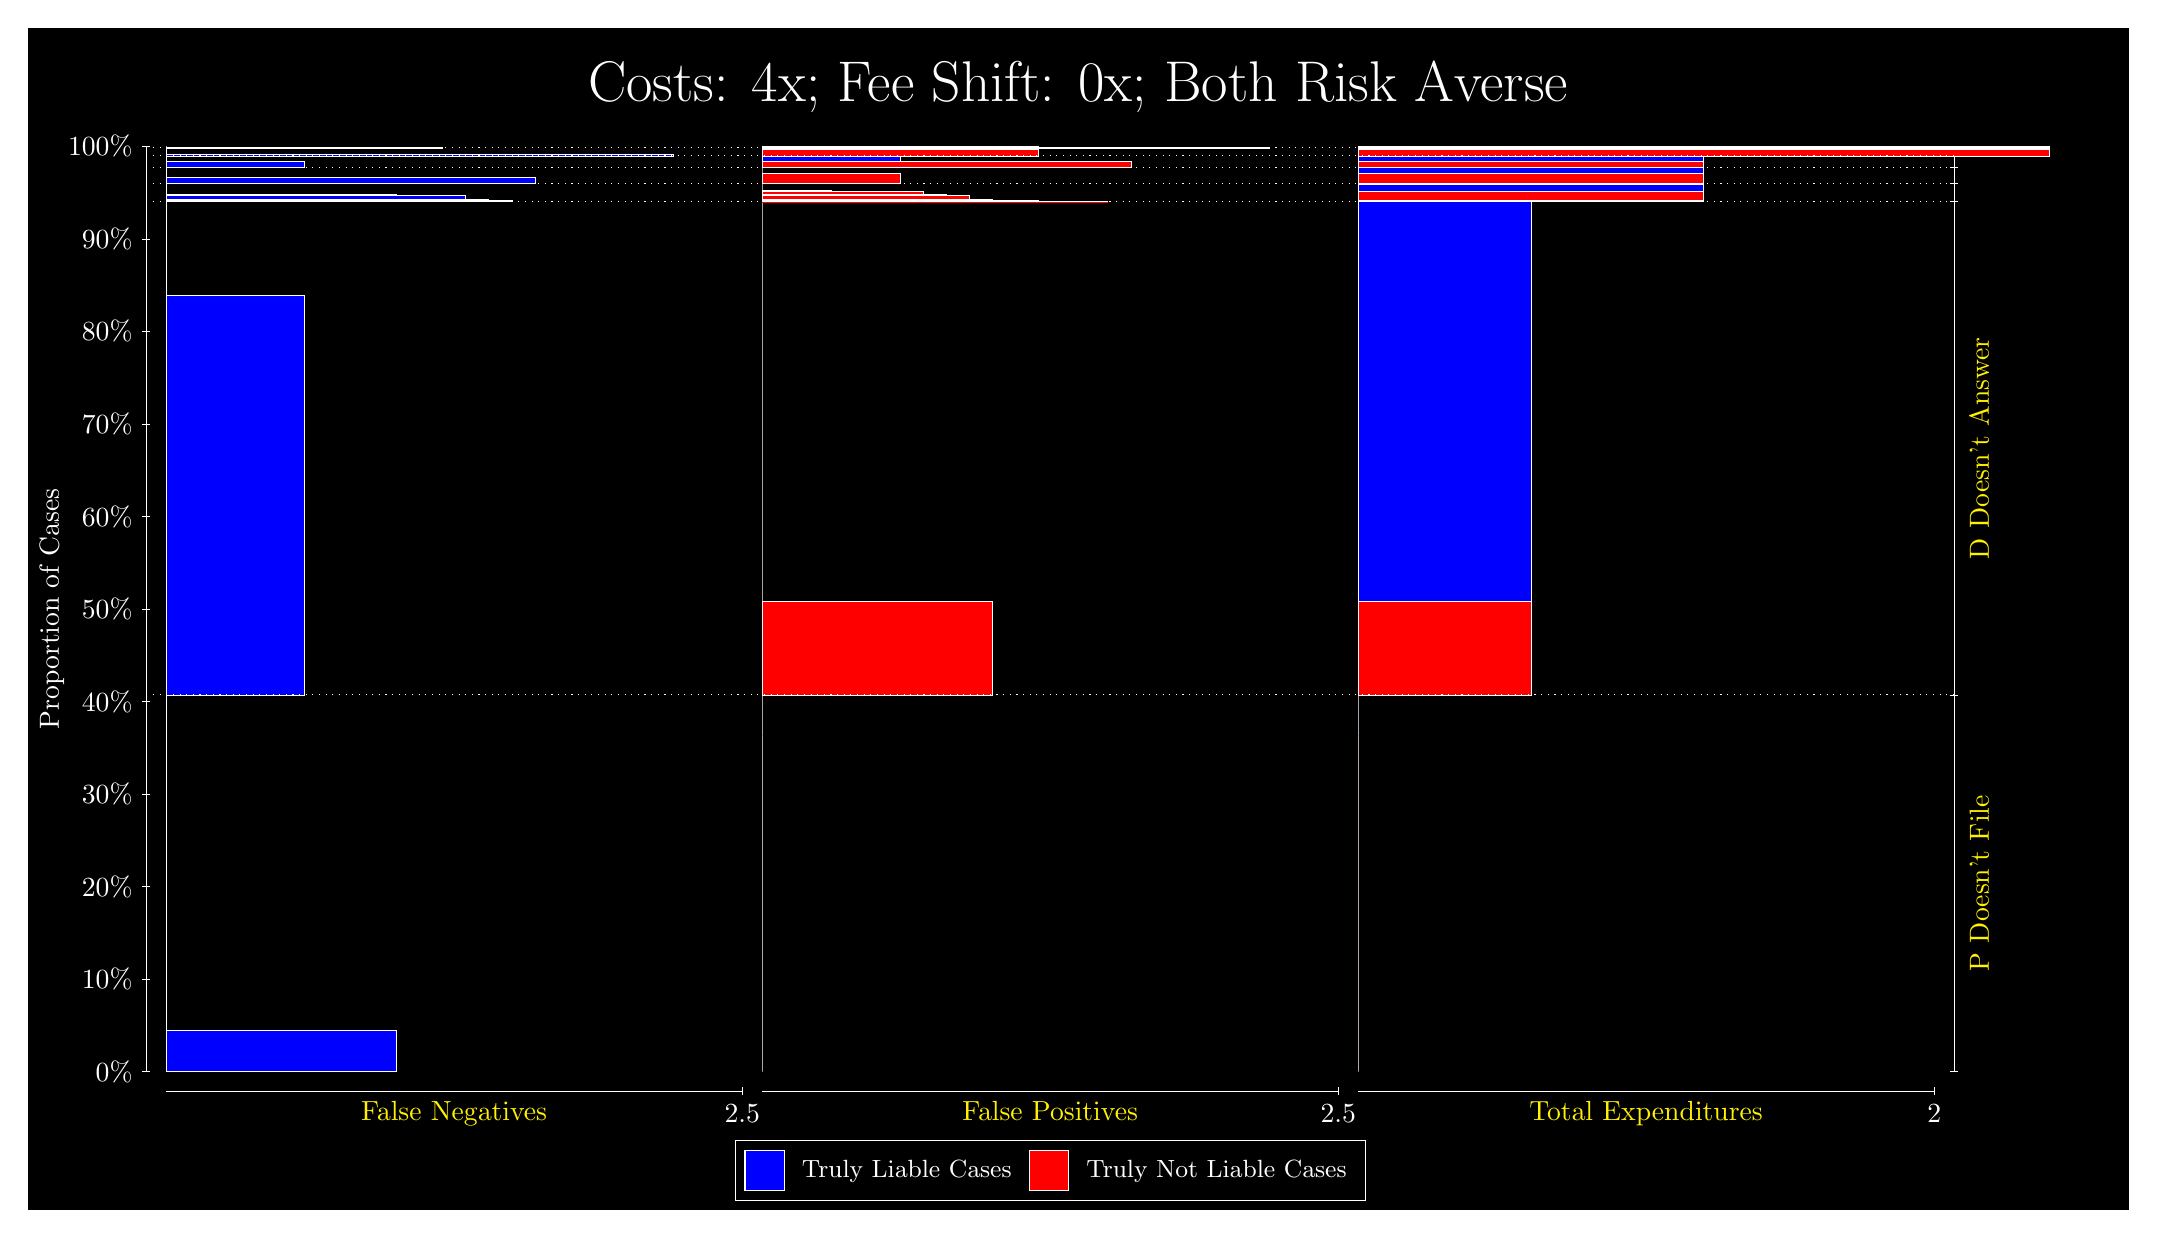
\begin{tikzpicture}
\draw[fill=black] (0,0) rectangle (26.667,15);
\draw[text=white] (0,13.5) rectangle (26.667,15) node[midway] {\huge Costs: 4x; Fee Shift: 0x; Both Risk Averse};
\draw[white, very thin] (1.5,1.75) -- (1.5,13.5);
\node[rotate=90, text=white, anchor=center] at (0.3, 7.625) {Proportion of Cases};
\draw[white, very thin] (1.45,1.75) -- (1.55,1.75);
\node[text=white, anchor=east] at (1.45, 1.75) {0\%};
\draw[white, very thin] (1.45,2.925) -- (1.55,2.925);
\node[text=white, anchor=east] at (1.45, 2.925) {10\%};
\draw[white, very thin] (1.45,4.1) -- (1.55,4.1);
\node[text=white, anchor=east] at (1.45, 4.1) {20\%};
\draw[white, very thin] (1.45,5.275) -- (1.55,5.275);
\node[text=white, anchor=east] at (1.45, 5.275) {30\%};
\draw[white, very thin] (1.45,6.45) -- (1.55,6.45);
\node[text=white, anchor=east] at (1.45, 6.45) {40\%};
\draw[white, very thin] (1.45,7.625) -- (1.55,7.625);
\node[text=white, anchor=east] at (1.45, 7.625) {50\%};
\draw[white, very thin] (1.45,8.8) -- (1.55,8.8);
\node[text=white, anchor=east] at (1.45, 8.8) {60\%};
\draw[white, very thin] (1.45,9.975) -- (1.55,9.975);
\node[text=white, anchor=east] at (1.45, 9.975) {70\%};
\draw[white, very thin] (1.45,11.15) -- (1.55,11.15);
\node[text=white, anchor=east] at (1.45, 11.15) {80\%};
\draw[white, very thin] (1.45,12.325) -- (1.55,12.325);
\node[text=white, anchor=east] at (1.45, 12.325) {90\%};
\draw[white, very thin] (1.45,13.5) -- (1.55,13.5);
\node[text=white, anchor=east] at (1.45, 13.5) {100\%};

\draw[white, very thin] (24.457,1.75) -- (24.457,13.5);
\draw[white, very thin] (24.407,1.75) -- (24.507,1.75);
\node[anchor=west] at (24.407, 1.75) {};
\draw[white, very thin] (24.407,6.5338) -- (24.507,6.5338);
\node[anchor=west] at (24.407, 6.5338) {};
\draw[white, very thin] (24.407,12.798) -- (24.507,12.798);
\node[anchor=west] at (24.407, 12.798) {};
\draw[white, very thin] (24.407,13.027) -- (24.507,13.027);
\node[anchor=west] at (24.407, 13.027) {};
\draw[white, very thin] (24.407,13.234) -- (24.507,13.234);
\node[anchor=west] at (24.407, 13.234) {};
\draw[white, very thin] (24.407,13.379) -- (24.507,13.379);
\node[anchor=west] at (24.407, 13.379) {};
\draw[white, very thin] (24.407,13.481) -- (24.507,13.481);
\node[anchor=west] at (24.407, 13.481) {};
\draw[white, very thin] (24.407,13.5) -- (24.507,13.5);
\node[anchor=west] at (24.407, 13.5) {};

\draw[white, very thin, fill=blue] (1.75,1.75) rectangle (4.6775,2.2685);
\draw[white, very thin, fill=red] (1.75,2.2685) rectangle (1.75,6.5338);
\draw[white, very thin, fill=blue] (1.75,6.5338) rectangle (3.5065,11.614);
\draw[white, very thin, fill=red] (1.75,11.614) rectangle (1.75,12.798);
\draw[white, very thin, fill=blue] (1.75,12.798) rectangle (6.1413,12.813);
\draw[white, very thin, fill=blue] (1.75,12.813) rectangle (5.8486,12.824);
\draw[white, very thin, fill=blue] (1.75,12.824) rectangle (5.5558,12.875);
\draw[white, very thin, fill=blue] (1.75,12.875) rectangle (5.2631,12.878);
\draw[white, very thin, fill=blue] (1.75,12.878) rectangle (4.9703,12.884);
\draw[white, very thin, fill=blue] (1.75,12.884) rectangle (4.6775,12.889);
\draw[white, very thin, fill=blue] (1.75,12.889) rectangle (4.3848,12.891);
\draw[white, very thin, fill=blue] (1.75,12.891) rectangle (4.092,12.892);
\draw[white, very thin, fill=blue] (1.75,12.892) rectangle (3.7993,12.893);
\draw[white, very thin, fill=red] (1.75,12.893) rectangle (1.75,13.027);
\draw[white, very thin, fill=blue] (1.75,13.027) rectangle (6.4341,13.104);
\draw[white, very thin, fill=red] (1.75,13.104) rectangle (1.75,13.234);
\draw[white, very thin, fill=blue] (1.75,13.234) rectangle (3.5065,13.307);
\draw[white, very thin, fill=red] (1.75,13.307) rectangle (1.75,13.379);
\draw[white, very thin, fill=blue] (1.75,13.379) rectangle (8.1906,13.402);
\draw[white, very thin, fill=red] (1.75,13.402) rectangle (1.75,13.481);
\draw[white, very thin, fill=blue] (1.75,13.481) rectangle (5.2631,13.491);
\draw[white, very thin, fill=red] (1.75,13.491) rectangle (1.75,13.5);
\draw[white, very thin, fill=red] (9.3189,1.75) rectangle (9.3189,6.0153);
\draw[white, very thin, fill=blue] (9.3189,6.0153) rectangle (9.3189,6.5338);
\draw[white, very thin, fill=red] (9.3189,6.5338) rectangle (12.246,7.7178);
\draw[white, very thin, fill=blue] (9.3189,7.7178) rectangle (9.3189,12.798);
\draw[white, very thin, fill=red] (9.3189,12.798) rectangle (13.71,12.799);
\draw[white, very thin, fill=red] (9.3189,12.799) rectangle (13.417,12.801);
\draw[white, very thin, fill=red] (9.3189,12.801) rectangle (13.125,12.805);
\draw[white, very thin, fill=red] (9.3189,12.805) rectangle (12.832,12.811);
\draw[white, very thin, fill=red] (9.3189,12.811) rectangle (12.539,12.819);
\draw[white, very thin, fill=red] (9.3189,12.819) rectangle (12.246,12.824);
\draw[white, very thin, fill=red] (9.3189,12.824) rectangle (11.954,12.882);
\draw[white, very thin, fill=red] (9.3189,12.882) rectangle (11.661,12.897);
\draw[white, very thin, fill=red] (9.3189,12.897) rectangle (11.368,12.933);
\draw[white, very thin, fill=blue] (9.3189,12.933) rectangle (10.783,12.934);
\draw[white, very thin, fill=blue] (9.3189,12.934) rectangle (10.49,12.934);
\draw[white, very thin, fill=blue] (9.3189,12.934) rectangle (10.197,12.937);
\draw[white, very thin, fill=blue] (9.3189,12.937) rectangle (9.9044,12.942);
\draw[white, very thin, fill=blue] (9.3189,12.942) rectangle (9.6116,12.947);
\draw[white, very thin, fill=blue] (9.3189,12.947) rectangle (9.3189,13.027);
\draw[white, very thin, fill=red] (9.3189,13.027) rectangle (11.075,13.158);
\draw[white, very thin, fill=blue] (9.3189,13.158) rectangle (9.3189,13.234);
\draw[white, very thin, fill=red] (9.3189,13.234) rectangle (14.003,13.307);
\draw[white, very thin, fill=blue] (9.3189,13.307) rectangle (11.075,13.379);
\draw[white, very thin, fill=red] (9.3189,13.379) rectangle (12.832,13.458);
\draw[white, very thin, fill=blue] (9.3189,13.458) rectangle (9.9044,13.481);
\draw[white, very thin, fill=red] (9.3189,13.481) rectangle (15.759,13.489);
\draw[white, very thin, fill=blue] (9.3189,13.489) rectangle (12.832,13.5);
\draw[white, very thin, fill=red] (16.888,1.75) rectangle (16.888,6.0153);
\draw[white, very thin, fill=blue] (16.888,6.0153) rectangle (16.888,6.5338);
\draw[white, very thin, fill=red] (16.888,6.5338) rectangle (19.083,7.7178);
\draw[white, very thin, fill=blue] (16.888,7.7178) rectangle (19.083,12.798);
\draw[white, very thin, fill=red] (16.888,12.798) rectangle (21.279,12.806);
\draw[white, very thin, fill=blue] (16.888,12.806) rectangle (21.279,12.812);
\draw[white, very thin, fill=red] (16.888,12.812) rectangle (21.279,12.933);
\draw[white, very thin, fill=blue] (16.888,12.933) rectangle (21.279,13.019);
\draw[white, very thin, fill=red] (16.888,13.019) rectangle (21.279,13.024);
\draw[white, very thin, fill=blue] (16.888,13.024) rectangle (21.279,13.027);
\draw[white, very thin, fill=red] (16.888,13.027) rectangle (21.279,13.158);
\draw[white, very thin, fill=blue] (16.888,13.158) rectangle (21.279,13.234);
\draw[white, very thin, fill=red] (16.888,13.234) rectangle (21.279,13.307);
\draw[white, very thin, fill=blue] (16.888,13.307) rectangle (21.279,13.379);
\draw[white, very thin, fill=red] (16.888,13.379) rectangle (25.67,13.458);
\draw[white, very thin, fill=blue] (16.888,13.458) rectangle (25.67,13.481);
\draw[white, very thin, fill=red] (16.888,13.481) rectangle (25.67,13.489);
\draw[white, very thin, fill=blue] (16.888,13.489) rectangle (25.67,13.5);
\draw[white, dotted] (1.5,6.5338) -- (24.457,6.5338);
\draw[white, dotted] (1.5,12.798) -- (24.457,12.798);
\draw[white, dotted] (1.5,13.027) -- (24.457,13.027);
\draw[white, dotted] (1.5,13.234) -- (24.457,13.234);
\draw[white, dotted] (1.5,13.379) -- (24.457,13.379);
\draw[white, dotted] (1.5,13.481) -- (24.457,13.481);
\draw[white, very thin] (1.75,1.5) -- (9.0689,1.5);
\node[text=yellow, anchor=north] at (5.4094, 1.5) {False Negatives};
\draw[white, very thin] (9.0689,1.45) -- (9.0689,1.55);
\node[text=white, anchor=north] at (9.0689, 1.45) {2.5};

\draw[white, very thin] (9.3189,1.5) -- (16.638,1.5);
\node[text=yellow, anchor=north] at (12.978, 1.5) {False Positives};
\draw[white, very thin] (16.638,1.45) -- (16.638,1.55);
\node[text=white, anchor=north] at (16.638, 1.45) {2.5};

\draw[white, very thin] (16.888,1.5) -- (24.207,1.5);
\node[text=yellow, anchor=north] at (20.547, 1.5) {Total Expenditures};
\draw[white, very thin] (24.207,1.45) -- (24.207,1.55);
\node[text=white, anchor=north] at (24.207, 1.45) {2};

\node[text=yellow, centered, rotate=90] at (24.777, 4.1419) {P Doesn't File};
\node[text=yellow, centered, rotate=90] at (24.777, 9.6661) {D Doesn't Answer};






\draw (12.978300999999998,1.5) node[draw=none] (baseCoordinate) {};
\begin{scope}[align=center]
        \matrix[scale=0.5, draw=white, below=0.5cm of baseCoordinate, nodes={draw}, column sep=0.1cm]{
            \node[rectangle, draw, minimum width=0.5cm, minimum height=0.5cm, fill=blue] {}; &
            \node[draw=none, font=\small, text=white] (B) {Truly Liable Cases}; &
            \node[rectangle, draw, minimum width=0.5cm, minimum height=0.5cm, fill=red] {}; &
            \node[draw=none, font=\small, text=white] (B) {Truly Not Liable Cases}; \\
            };
\end{scope}

\end{tikzpicture}
\end{document}